% =====================================================================
%  M.Tech Thesis Defense — Adarsh Dubey (SC24M151)
%  Title : High-Performance Deep Learning Software Stack for
%          Scalable and Efficient LLMs
%  Target: 40 slides, 25--30 minutes
% =====================================================================
\documentclass[10pt,aspectratio=169]{beamer}

\usetheme{Madrid}
\usecolortheme{seahorse}
\useinnertheme{rectangles}
\useoutertheme{infolines}
\setbeamertemplate{navigation symbols}{}
\setbeamertemplate{caption}[numbered]

\usepackage[T1]{fontenc}
\usepackage{lmodern}
\usepackage{amsmath,amssymb,amsthm,mathtools}
\usepackage{booktabs}
\usepackage{multirow}
\usepackage{tikz}
\usepackage{pgfplots}
\pgfplotsset{compat=1.16}
\usetikzlibrary{shapes,arrows,positioning,matrix,patterns,calc,fit,
                backgrounds,decorations.pathreplacing}
\usepackage[ruled,vlined,linesnumbered]{algorithm2e}
\usepackage{subcaption}
\usepackage{listings}

\lstset{
  basicstyle=\ttfamily\scriptsize,
  breaklines=true,
  frame=single,
  numbers=left,
  numberstyle=\tiny,
  keywordstyle=\color{blue!70!black},
  commentstyle=\color{green!50!black}\itshape,
}

\newtheorem{thm}{Theorem}
\newtheorem{lem}{Lemma}

% --- Title metadata ---------------------------------------------------
\title[HPC-DL Stack for LLMs]%
      {High-Performance Deep Learning\\Software Stack for Scalable and
       Efficient LLMs}
\subtitle{M.\,Tech Thesis Defense}
\author[Adarsh Dubey]{Adarsh Dubey \\ \scriptsize SC24M151}
\institute[IIST]{Department of Mathematics\\
                 Indian Institute of Space Science and Technology\\
                 Advisor: Dr.~S.~Sumitra}
\date{\today}

% =====================================================================
\begin{document}
% =====================================================================

% --------------------------- 1. Title --------------------------------
\begin{frame}[plain]
  \titlepage
\end{frame}

% --------------------------- 2. TL;DR --------------------------------
\begin{frame}{At a Glance}
  \textbf{One-line thesis}: co-design every layer of the LLM stack so
  the savings compose, then measure it.
  \vspace{1.5ex}

  \textbf{Headline numbers} (8$\times$A100-40GB):
  \begin{itemize}
    \item \alert{93.8\%} peak GPU utilisation with DeepSpeed ZeRO-3
          ($\approx 87.5\%$ memory reduction over DP)
    \item \alert{65.6\%} attention blocks skipped by SWFA with
          $<\!10^{-4}$ FP32 error
    \item \alert{50--59\%} end-to-end training speedup on GPT-2-Medium
    \item \alert{2.84$\times$} decode throughput on LLaMA-7B via the
          SGLang kernel stack
    \item \alert{25--29\%} energy savings per epoch
  \end{itemize}
  \vspace{1ex}
  \textbf{Talk plan}: motivation $\to$ 5 layers $\to$ SWFA deep dive $\to$
  serving $\to$ conclusions.
\end{frame}

% --------------------------- 3. Problem ------------------------------
\begin{frame}{The Problem}
  Training and serving modern LLMs stresses \emph{every} layer at once:
  \begin{itemize}
    \item \textbf{Schedule} — $10^3$ accelerators must stay in lockstep.
    \item \textbf{Kernel} — GEMMs must saturate Tensor Cores.
    \item \textbf{Algorithm} — attention must scale sub-quadratically with
          the context window $N$.
    \item \textbf{Runtime} — decode must turn savings into tokens/s
          under latency SLOs.
    \item \textbf{Tooling} — every kernel needs a roofline and an
          auto-tuner.
  \end{itemize}
  \vspace{1ex}
  \alert{Isolated optimisations leave the gains of the others on the
         table.}
  \vspace{2ex}

  This thesis builds an \emph{end-to-end} stack in which the five
  layers are designed to \emph{compose}, and measures it.
\end{frame}

% --------------------------- 4. Stack overview -----------------------
\begin{frame}{The Five-Layer Stack}
  \centering
  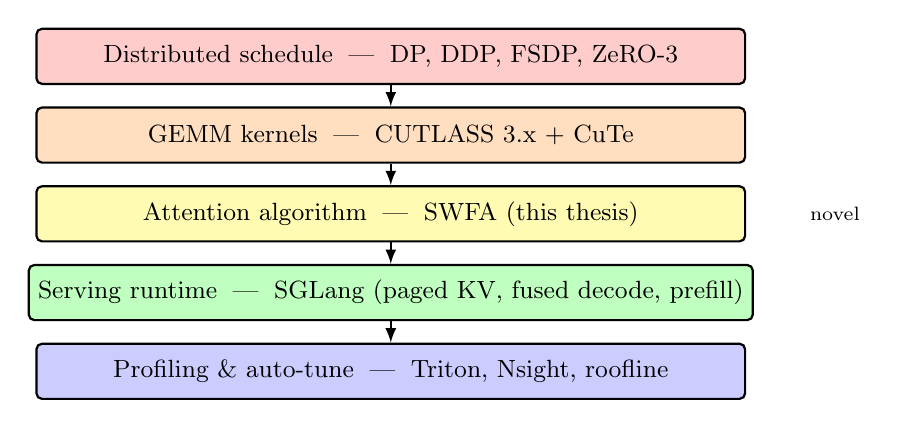
\begin{tikzpicture}[
      layer/.style={rectangle, rounded corners=2pt, draw=black,
                    thick, minimum width=9cm, minimum height=7mm,
                    font=\small},
      arrow/.style={-latex, thick}
  ]
    \node[layer, fill=red!20]    (a) at (0, 4)  {Distributed schedule \;—\; DP, DDP, FSDP, ZeRO-3};
    \node[layer, fill=orange!25] (b) at (0, 3)  {GEMM kernels \;—\; CUTLASS 3.x + CuTe};
    \node[layer, fill=yellow!30] (c) at (0, 2)  {Attention algorithm \;—\; \alert{SWFA (this thesis)}};
    \node[layer, fill=green!25]  (d) at (0, 1)  {Serving runtime \;—\; SGLang (paged KV, fused decode, prefill)};
    \node[layer, fill=blue!20]   (e) at (0, 0)  {Profiling \& auto-tune \;—\; Triton, Nsight, roofline};
    \draw[arrow] (a) -- (b);
    \draw[arrow] (b) -- (c);
    \draw[arrow] (c) -- (d);
    \draw[arrow] (d) -- (e);
    \node[font=\scriptsize, anchor=west] at (5.2, 2) {novel};
  \end{tikzpicture}
  \vspace{1ex}

  Clean interfaces; each layer's output is the next layer's input.
\end{frame}

% --------------------------- 5. Contributions ------------------------
\begin{frame}{Contributions}
  \begin{enumerate}
    \item Controlled 8-GPU study of DP/DDP/FSDP/ZeRO-3 with identical
          seeds and workload; 22\% lower energy per epoch for ZeRO-3.
    \item CUTLASS/CuTe mapping of LLM GEMMs (QKV, attention-score,
          MLP, MoE) with epilogue fusion — up to 35\% speedup on skinny
          shapes.
    \item \alert{SWFA}: block-sparse Sliding Window Flash Attention
          with vectorised mask, corner-check lemma, and a
          \emph{closed-form optimal window} under an exponential-decay
          cost model (strict convexity proved).
    \item SGLang kernel stack: paged KV + fused decode + SWFA prefill
          + fused sampling $\Rightarrow$ $2.84\times$ on LLaMA-7B.
    \item Triton profiling/auto-tuning pipeline; cross-validates
          CUTLASS and Torch-inductor within $<\!3\%$.
  \end{enumerate}
\end{frame}

% --------------------------- 6. Roadmap ------------------------------
\begin{frame}{Talk Roadmap}
  \begin{columns}[T]
    \begin{column}{0.5\textwidth}
      \textbf{Part I — Foundations} \hfill (\S2, \S3)\\[0.5ex]
      \footnotesize literature $\cdot$ distributed training study
      \vspace{2ex}

      \textbf{Part II — Kernels} \hfill (\S4)\\[0.5ex]
      \footnotesize CUTLASS + CuTe GEMMs
      \vspace{2ex}

      \textbf{Part III — Algorithm} \hfill (\S5)\\[0.5ex]
      \footnotesize \alert{Sliding Window Flash Attention (SWFA)}
    \end{column}
    \begin{column}{0.5\textwidth}
      \textbf{Part IV — Serving} \hfill (\S6)\\[0.5ex]
      \footnotesize SGLang kernel stack
      \vspace{2ex}

      \textbf{Part V — Tooling} \hfill (\S7)\\[0.5ex]
      \footnotesize Triton profiling \& auto-tune
      \vspace{2ex}

      \textbf{Part VI — Wrap} \hfill (\S8)\\[0.5ex]
      \footnotesize lessons, limitations, future work
    \end{column}
  \end{columns}
\end{frame}

% =====================================================================
%  Part I — Foundations
% =====================================================================

% --------------------------- 7. Prior art ----------------------------
\begin{frame}{Prior Art at Each Layer}
  \small
  \begin{tabular}{ll}
    \toprule
    \textbf{Layer} & \textbf{Representative prior work} \\
    \midrule
    Distributed   & ZeRO (Rajbhandari'20), FSDP (Zhao'23), Megatron-LM \\
    GEMM kernels  & CUTLASS, CuTe, cuBLAS, Triton \\
    Attention     & Flash Attention 1/2 (Dao'22/'23), Longformer, BigBird \\
    Serving       & vLLM (paged attention), SGLang, TGI \\
    Profiling     & Nsight Compute, NVTX, Triton benchmark harness \\
    \bottomrule
  \end{tabular}
  \vspace{2ex}

  \textbf{Observation}: each layer has strong isolated work, but the
  interfaces between them are ad-hoc. No prior work reports a
  \emph{controlled} five-layer study on the same hardware.
\end{frame}

% --------------------------- 8. Positioning --------------------------
\begin{frame}{Where This Thesis Sits}
  \textbf{What is new}:
  \begin{itemize}
    \item A \emph{controlled} 4-way distributed study on one node
          (identical seeds, workload, initialisation).
    \item A block-classification step \emph{in front} of Flash
          Attention that skips entire $B_r{\times}B_c$ blocks.
    \item A closed-form optimal window $w^\star$ with a convexity
          proof.
    \item A layered evaluation of five SGLang kernel optimisations
          that attributes the cumulative $2.84\times$ to each layer.
  \end{itemize}
  \vspace{2ex}

  \textbf{What is deliberately out of scope}:
  multi-node scaling, sub-8-bit quantisation, RLHF workloads.
\end{frame}

% =====================================================================
%  Part II — Distributed Training
% =====================================================================

% --------------------------- 9. Four strategies ----------------------
\begin{frame}{Four Distributed Strategies}
  \footnotesize
  \begin{tabular}{@{}lcccc@{}}
    \toprule
    & \textbf{Params} & \textbf{Grads} & \textbf{Optim.} & \textbf{Comms}\\
    \midrule
    DP             & replicated & replicated & replicated & scatter/gather\\
    DDP            & replicated & \alert{ring-reduced} & replicated & all-reduce\\
    FSDP           & \alert{sharded} & \alert{sharded} & \alert{sharded} & gather $\to$ compute $\to$ shard\\
    ZeRO-3         & \alert{sharded} & \alert{sharded} & \alert{sharded} & fine-grained overlap\\
    \bottomrule
  \end{tabular}
  \vspace{2ex}

  \textbf{Trade-off}: replication $\Rightarrow$ fewer comms but higher
  memory; sharding $\Rightarrow$ $P\times$ memory reduction but extra
  gather/scatter.
  \vspace{1ex}

  \textbf{Goal}: isolate the effect of the \emph{strategy itself},
  not the framework or workload.
\end{frame}

% --------------------------- 10. Memory math -------------------------
\begin{frame}{Memory Partitioning Math}
  Let $M$ be model parameters, $P$ GPUs, $B$ per-GPU batch.
  Per-GPU memory for each strategy:
  \begin{align*}
  \text{DP, DDP}  &: \quad M_{\text{param}} + M_{\text{grad}} + M_{\text{opt}} + M_{\text{act}}(B)\\
  \text{FSDP}     &: \quad \tfrac{1}{P}\bigl(M_{\text{param}} + M_{\text{grad}} + M_{\text{opt}}\bigr) + M_{\text{act}}(B)\\
  \text{ZeRO-3}   &: \quad \tfrac{1}{P}\bigl(M_{\text{param}} + M_{\text{grad}} + M_{\text{opt}}\bigr) + M_{\text{act}}(B) + M_{\text{bucket}}
  \end{align*}
  For Adam on $P{=}8$, the savings factor is $87.5\%$ on the
  param+grad+opt sum; activation memory is unchanged.
  \vspace{2ex}

  \textbf{Comms cost per step} (ring all-reduce, $\tau$ latency,
  $1/\beta$ bandwidth):
  \[
    T_{\text{AR}}(M) = 2(P{-}1)\!\left(\tau + \tfrac{M}{P\beta}\right)
    \;\xrightarrow[P\to\infty]{} \; \tfrac{2M}{\beta}.
  \]
\end{frame}

% --------------------------- 11. Methodology -------------------------
\begin{frame}{Experimental Methodology}
  \begin{columns}[T]
    \begin{column}{0.5\textwidth}
      \textbf{Hardware}: 8$\times$ A100-40GB on one node,
      NVLink, CUDA 12.x, NCCL 2.19.

      \textbf{Workload (training)}: ResNet-50 / CIFAR-10
      (controlled proxy), GPT-2 Medium (355M)
      for LLM runs.

      \textbf{Seeds}: fixed across strategies, framework, and
      kernels.
    \end{column}
    \begin{column}{0.5\textwidth}
      \textbf{Metrics}
      \begin{itemize}\footnotesize
        \item GPU util (avg / peak)
        \item Per-GPU memory (model / grad / opt)
        \item Training-loss convergence
        \item Power and energy per epoch
        \item Compute/comms overlap
        \item Throughput scaling
      \end{itemize}
    \end{column}
  \end{columns}
  \vspace{2ex}
  \centering
  \alert{Same code path; only the strategy varies.}
\end{frame}

% --------------------------- 12. Results util ------------------------
\begin{frame}{Results — GPU Utilisation \& Memory}
  \begin{columns}[T]
    \begin{column}{0.54\textwidth}
      \centering\scriptsize
      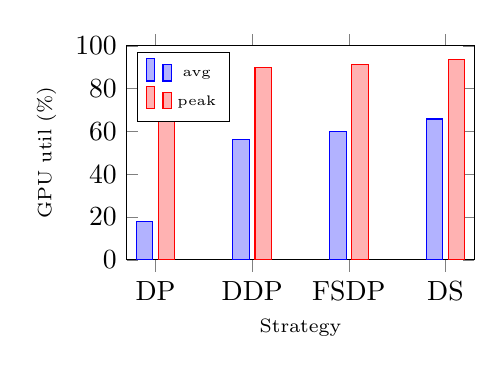
\begin{tikzpicture}
        \begin{axis}[
            ybar, width=6cm, height=4.3cm,
            xlabel=\scriptsize Strategy, ylabel=\scriptsize GPU util (\%),
            ymin=0, ymax=100, xtick=data,
            xticklabels={DP,DDP,FSDP,DS},
            bar width=6pt, legend style={font=\tiny},
            legend pos=north west]
          \addplot coordinates {(0,18.13)(1,56.2)(2,60.15)(3,65.8)};
          \addplot coordinates {(0,72.3)(1,89.7)(2,91.2)(3,93.8)};
          \legend{avg, peak}
        \end{axis}
      \end{tikzpicture}
    \end{column}
    \begin{column}{0.46\textwidth}
      \scriptsize
      \begin{tabular}{@{}lcc@{}}
        \toprule
        \textbf{Strategy} & \textbf{Mem/GPU (GB)} & \textbf{Reduction}\\
        \midrule
        DP  & 3.92 & 1.0$\times$\\
        DDP & 3.92 & 1.0$\times$\\
        FSDP & 0.49 & \alert{8.0$\times$}\\
        ZeRO-3 & 0.49 & \alert{8.0$\times$}\\
        \bottomrule
      \end{tabular}
      \vspace{1ex}

      \footnotesize
      ZeRO-3 peaks at \alert{93.8\%} via fine-grained overlap of
      parameter gather with compute. Sharding delivers the
      theoretical $\approx 87.5\%$ memory saving.
    \end{column}
  \end{columns}
\end{frame}

% --------------------------- 13. Results energy ----------------------
\begin{frame}{Results — Energy \& Communication Overlap}
  \footnotesize
  \begin{tabular}{@{}lcccc@{}}
    \toprule
    \textbf{Strategy} & \textbf{Avg (W)} & \textbf{kWh/epoch}
                      & \textbf{Comms} & \textbf{Overlap (\%)}\\
    \midrule
    DP              & 2\,840 & 0.95 & poor       & 12\\
    DDP             & 2\,720 & 0.87 & good       & 64\\
    FSDP            & 2\,650 & 0.82 & good       & 58\\
    DeepSpeed       & 2\,580 & 0.78 & \alert{excellent} & 61\\
    \bottomrule
  \end{tabular}
  \vspace{2ex}

  \begin{itemize}
    \item ZeRO-3 delivers \alert{22\%} lower per-epoch energy than DP
          at the \emph{same} final loss.
    \item DDP overlaps best: ring all-reduce runs \emph{concurrently}
          with the backward pass of earlier layers.
    \item ZeRO-3's explicit parameter-gather phase blocks compute
          slightly; \texttt{overlap\_comm} partially hides it.
  \end{itemize}
\end{frame}

% =====================================================================
%  Part III — CUTLASS / CuTe
% =====================================================================

% --------------------------- 14. CUTLASS hierarchy -------------------
\begin{frame}{CUTLASS \& CuTe — The Tile Hierarchy}
  Three nested tilings of a GEMM $C = A\cdot B$:
  \begin{enumerate}
    \item \textbf{Threadblock tile} $(M_{tb}, N_{tb}, K_{tb})$
          — unit of HBM traffic.
    \item \textbf{Warp tile}       $(M_w, N_w, K_w)$
          — unit of shared-memory traffic.
    \item \textbf{Instruction tile} $(M_i, N_i, K_i)$
          — Tensor Core MMA shape, e.g. $16{\times}8{\times}16$.
  \end{enumerate}
  \vspace{1ex}
  \textbf{CuTe layouts} express these tilings as tuples
  $\texttt{Shape}\;\oplus\;\texttt{Stride}$, and composition makes the
  tiling explicit:
  \[
    \texttt{Layout}(S,D) \circ \texttt{Layout}(S', D')
      \;=\; \texttt{Layout}\bigl((S, S'),\; (D\cdot D', D')\bigr).
  \]
  \vspace{-1ex}

  \textbf{Multi-stage pipelining}: prefetch tile $k{+}1$ into shared
  memory while MMAs on tile $k$ execute, typically 3 stages for
  square GEMM, 2 for skinny GEMM.
\end{frame}

% --------------------------- 15. Epilogue fusion ---------------------
\begin{frame}{Epilogue Fusion}
  \textbf{Without fusion}: three HBM round-trips.
  \[
    Y \leftarrow W X;\quad Z \leftarrow Y + b;\quad Z \leftarrow \phi(Z).
  \]
  \textbf{With fusion}: one HBM round-trip.
  \[
    Z_{ij} \leftarrow \phi\!\Bigl(\textstyle\sum_k W_{ik} X_{kj} + b_i\Bigr).
  \]
  \vspace{1ex}
  Bias and activation ($\phi$) are executed \emph{in register} after
  the final MMA accumulation, before the store to HBM.
  \vspace{2ex}

  \textbf{Impact on GPT-2-Medium MLP}:
  \begin{itemize}
    \item Bias+GELU fused into FC1: \alert{18\%} faster at $N{=}2048$.
    \item Residual-add fused into FC2: \alert{22\%} faster at $N{=}4096$.
  \end{itemize}
  Savings come entirely from eliminated HBM passes.
\end{frame}

% --------------------------- 16. CUTLASS results ---------------------
\begin{frame}{Results — CUTLASS vs.\ cuBLAS}
  \footnotesize
  \begin{tabular}{@{}lcccc@{}}
    \toprule
    \textbf{Shape ($M{\times}N{\times}K$)} & \textbf{Dtype}
    & \textbf{cuBLAS} & \textbf{CUTLASS} & \textbf{Ratio}\\
    \midrule
    $4096^3$                      & FP16 & 280 & 301 & 1.08$\times$\\
    $8192^3$                      & FP16 & 305 & 318 & 1.04$\times$\\
    $2048\times2048\times128$ (skinny) & FP16 & 95  & 128 & \alert{1.35$\times$}\\
    Grouped MoE, 16 experts       & FP16 & 184 & 241 & \alert{1.31$\times$}\\
    \bottomrule
  \end{tabular}
  \vspace{2ex}

  \begin{itemize}
    \item CUTLASS matches cuBLAS on \emph{large} shapes — both are
          compute-bound with Tensor Core util $>90\%$.
    \item CUTLASS beats cuBLAS on \emph{skinny} and \emph{grouped}
          GEMMs — exactly the shapes that dominate attention and MoE.
    \item $35\%$ win on $2048{\times}2048{\times}128$ comes from a
          warp tile of $64{\times}32{\times}32$ matching register
          budget per warp.
  \end{itemize}
\end{frame}

% =====================================================================
%  Part IV — SWFA (10 slides) — CENTERPIECE
% =====================================================================

% --------------------------- 17. SWFA motivation ---------------------
\begin{frame}{SWFA — Motivation}
  Standard attention is quadratic:
  \[
     \mathrm{Attn}(Q,K,V) =
     \mathrm{softmax}\!\left(\frac{QK^{\!\top}}{\sqrt{d}}\right) V,
     \qquad \text{cost} = \Theta(N^2 d).
  \]
  \vspace{-1ex}
  \begin{itemize}
    \item Flash Attention 1/2 fix the \emph{memory} wall but still
          issue dense GEMMs on every $B_r{\times}B_c$ tile.
    \item Many long-context models (Longformer, BigBird,
          Mistral-7B) restrict attention to a \emph{local window}
          $[i-w_l, i+w_r]$ — a hard architectural constraint.
    \item Theory says cost drops from $\Theta(N^2)$ to $\Theta(Nw)$,
          but only if the kernel itself is window-aware.
  \end{itemize}
  \vspace{1ex}

  \alert{SWFA = Flash Attention + explicit block classification +
         vectorised mask.}
\end{frame}

% --------------------------- 18. Online softmax ----------------------
\begin{frame}{Flash Attention's Online Softmax}
  Partition $Q$ into row tiles of height $B_r$, $K,V$ into column
  tiles of width $B_c$. For row block $i$, maintain a running
  $(m_i, \ell_i, O_i) = $ (row-max, row-sum, output accumulator):
  \[
    m_i^{\text{new}} = \max\!\bigl(m_i,\; \max_j s_{ij}\bigr),
  \]
  \[
    \ell_i^{\text{new}} = e^{m_i - m_i^{\text{new}}}\,\ell_i
                          + \sum_j e^{s_{ij} - m_i^{\text{new}}},
  \]
  \[
    O_i^{\text{new}} = e^{m_i - m_i^{\text{new}}}\,O_i
                          + \sum_j e^{s_{ij} - m_i^{\text{new}}} v_j.
  \]
  \vspace{0.5ex}

  \textbf{Result}: peak HBM residency drops from $\Theta(N^2)$ to
  $\Theta(B_r B_c)$ without changing the mathematical answer (up to
  FP associativity).\\[0.5ex]
  \textbf{Key insight}: an identical $(m, \ell, O)$ state-machine
  works \emph{block-by-block} — so we can \alert{skip blocks} that
  contribute nothing.
\end{frame}

% --------------------------- 19. Block classification fig ------------
\begin{frame}{Block Classification: $\mathcal{I}$ / $\mathcal{X}$ / $\mathcal{O}$}
  \centering
  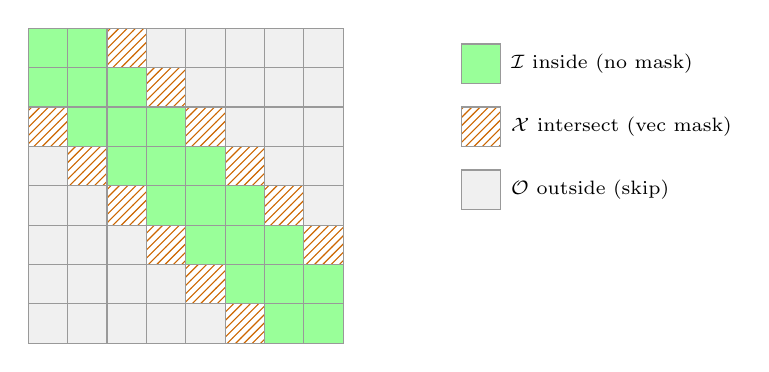
\begin{tikzpicture}[
      cell/.style={minimum width=5mm, minimum height=5mm, draw=black!40,
                   inner sep=0pt, font=\tiny},
      inside/.style ={cell, fill=green!40},
      inter/.style  ={cell, fill=orange!50,
                      pattern=north east lines, pattern color=orange!80!black},
      outside/.style={cell, fill=gray!12}]
    \foreach \i in {0,...,7} {
      \foreach \j in {0,...,7} {
        \pgfmathtruncatemacro{\diff}{abs(\i - \j)}
        \ifnum\diff=0
          \node[inside]  at (\j*5mm, -\i*5mm) {};
        \else\ifnum\diff=1
          \node[inside]  at (\j*5mm, -\i*5mm) {};
        \else\ifnum\diff=2
          \node[inter]   at (\j*5mm, -\i*5mm) {};
        \else
          \node[outside] at (\j*5mm, -\i*5mm) {};
        \fi\fi\fi
      }
    }
    \node[inside,  label=right:{\scriptsize $\mathcal{I}$ inside (no mask)}]
        at (55mm,   -2mm) {};
    \node[inter,   label=right:{\scriptsize $\mathcal{X}$ intersect (vec mask)}]
        at (55mm,  -10mm) {};
    \node[outside, label=right:{\scriptsize $\mathcal{O}$ outside (\alert{skip})}]
        at (55mm, -18mm) {};
  \end{tikzpicture}

  \vspace{1ex}
  \footnotesize Example: $N{=}8$, $w_l{=}w_r{=}2$. Asymptotic skipped
  fraction $\to 1 - 2w/N$.
\end{frame}

% --------------------------- 20. Classification algo -----------------
\begin{frame}{Classification Algorithm (corner check)}
  \scriptsize
  \begin{algorithm}[H]
    \SetAlgoLined
    \KwIn{$N$, window $(w_l, w_r)$, block sizes $(B_r, B_c)$.}
    \KwOut{sets $\mathcal{I}, \mathcal{X}, \mathcal{O}$.}
    $T_r \leftarrow \lceil N/B_r \rceil$,\ $T_c \leftarrow \lceil N/B_c \rceil$\;
    \For{$r = 0$ \KwTo $T_r - 1$}{
      $r_0 \leftarrow rB_r$,\ $r_1 \leftarrow \min((r{+}1)B_r, N){-}1$\;
      \For{$c = 0$ \KwTo $T_c - 1$}{
        $c_0 \leftarrow cB_c$,\ $c_1 \leftarrow \min((c{+}1)B_c, N){-}1$\;
        $\textit{outside} \leftarrow (c_1 < r_0 - w_l) \lor (c_0 > r_1 + w_r)$\;
        $\textit{inside} \leftarrow (c_1 \le r_0 + w_r) \land (c_0 \ge r_1 - w_l)$\;
        \uIf{outside}{$\mathcal{O} \mathrel{{+}{=}} \{(r,c)\}$}
        \uElseIf{inside}{$\mathcal{I} \mathrel{{+}{=}} \{(r,c)\}$}
        \Else{$\mathcal{X} \mathrel{{+}{=}} \{(r,c)\}$}
      }
    }
    \Return $(\mathcal{I}, \mathcal{X}, \mathcal{O})$
  \end{algorithm}
  \vspace{0.5ex}\normalsize
  Cost: $\mathcal{O}(T_rT_c) = \mathcal{O}((N/B)^2)$, dominated by the
  $\mathcal{O}(Nw/B)$ non-skipped kernel work.
\end{frame}

% --------------------------- 21. Corner lemma ------------------------
\begin{frame}{Corner-Check Sufficiency (Lemma)}
  \begin{lem}[Corner-check sufficiency]
  Let $B = [r_0,r_1] \times [c_0, c_1]$ be a block and
  $W = \{(i,j) : i - w_l \le j \le i + w_r\}$ the window. Then
  \begin{enumerate}
    \item[\textup{(i)}]
      $B \cap W = \emptyset \iff c_1 < r_0 - w_l$ \emph{or}
                              $c_0 > r_1 + w_r$;
    \item[\textup{(ii)}]
      $B \subseteq W \iff c_1 \le r_0 + w_r$ \emph{and}
                              $c_0 \ge r_1 - w_l$.
  \end{enumerate}
  \end{lem}
  \textbf{Proof sketch.} Window boundaries $j = i \pm w_r,\, j = i - w_l$ are
  monotone in $i$, so $\min_{(i,j)\in B}(j-i)$ is attained at
  $(r_1, c_0)$ and $\max$ at $(r_0, c_1)$. Outside / inside reduce to
  inequalities on these two corners. $\square$
  \vspace{1ex}

  \textbf{Consequence}: classification needs only \alert{4
  comparisons per block} — trivial runtime overhead.
\end{frame}

% --------------------------- 22. Vectorised mask ---------------------
\begin{frame}{Vectorised Mask Generation for $\mathcal{X}$}
  For block $(r,c)$ let $\delta_{rc} = cB_c - rB_r$. A local offset
  $\text{rel} = j_\ell - i_\ell$ must be masked iff
  \[
    \text{rel} > w_r + \delta_{rc}
    \;\; \text{or}\;\;
    \text{rel} < -w_l + \delta_{rc}.
  \]
  Define diagonals
  \[
    d_{\text{right}} = \lfloor w_r + \delta_{rc}\rfloor + 1,\qquad
    d_{\text{left}}  = \lfloor -w_l + \delta_{rc}\rfloor - 1.
  \]
  Then the mask is a single vectorised expression:
  \[
    M_{rc} =
     \mathrm{triu}\bigl(\mathbf{1}_{B_r \times B_c},\ d_{\text{right}}\bigr)
     \;\lor\;
     \mathrm{tril}\bigl(\mathbf{1}_{B_r \times B_c},\ d_{\text{left}}\bigr).
  \]
  Replaces a nested $\mathcal{O}(B_r B_c)$ Python loop with a single
  \texttt{triu/tril} call; \alert{$\sim$100$\times$} faster than naive
  masking at the block level.
\end{frame}

% --------------------------- 23. SWFA forward algo -------------------
\begin{frame}{SWFA Forward Algorithm}
  \scriptsize
  \begin{algorithm}[H]
    \SetAlgoLined
    \KwIn{$Q \in \mathbb{R}^{B\times H\times N\times d}$,
          $K,V \in \mathbb{R}^{B\times H\times N\times d_v}$,
          $(w_l, w_r)$, $(B_r, B_c)$.}
    $(\mathcal{I},\mathcal{X},\mathcal{O}) \leftarrow \textsc{ClassifyBlocks}$\;
    \For{$r = 0$ \KwTo $T_r-1$}{
      $O_r \leftarrow 0,\; m_r \leftarrow -\infty,\; \ell_r \leftarrow 0$\;
      \For{$c = 0$ \KwTo $T_c-1$}{
        \If{$(r,c) \in \mathcal{O}$}{\textbf{continue}\ \tcp*{skip block}}
        $S_{rc} \leftarrow Q_r K_c^{\!\top} / \sqrt{d}$\;
        \If{$(r,c) \in \mathcal{X}$}{$S_{rc} \mathrel{{+}{=}} \textsc{GenerateMask}$}
        $m_r^{\text{new}} \leftarrow \max(m_r, \max S_{rc})$;\;
        $\text{corr} \leftarrow e^{m_r - m_r^{\text{new}}}$;\;
        $P_{rc} \leftarrow e^{S_{rc} - m_r^{\text{new}}}$;\;
        $\ell_r \leftarrow \text{corr}\cdot\ell_r + \sum P_{rc}$;\;
        $O_r \leftarrow \text{corr}\cdot O_r + P_{rc}V_c$;\;
        $m_r \leftarrow m_r^{\text{new}}$\;
      }
      $O_r \leftarrow O_r / (\ell_r + \varepsilon)$\;
    }
    \Return $O$
  \end{algorithm}
\end{frame}

% --------------------------- 24. Backward + complexity ---------------
\begin{frame}{Backward Pass \& Complexity}
  \textbf{Backward} re-runs the forward loop over the \emph{same}
  block set $\mathcal{I}\cup\mathcal{X}$. Using stored $(m_r,\ell_r)$:
  \[
     P_{rc} = e^{S_{rc} - m_r}/\ell_r,\quad
     \mathrm{d}S_{rc} = P_{rc}\odot(\mathrm{d}P_{rc} - \rho_r),
  \]
  with $\rho_r = \sum_c P_{rc}\odot(\mathrm{d}O_r V_c^{\!\top})$. No
  extra memory vs.\ FA; skipped blocks contribute zero.

  \vspace{1.5ex}
  \textbf{Complexity} (sequence $N$, window $w$, block $B$):
  \begin{center}
  \begin{tabular}{@{}lc@{}}
    \toprule
    Total blocks             & $(N/B)^2$\\
    Inside band $(\mathcal{I} \cup \mathcal{X})$  & $\approx 2(N/B)(w/B)$\\
    Skipped ($\mathcal{O}$) & $(N/B)^2 - 2(N/B)(w/B)$\\
    \alert{Theoretical speedup} & $1 - 2w/N$ (as $w \ll N$)\\
    Memory & $\Theta(N)$ (same as FA)\\
    \bottomrule
  \end{tabular}
  \end{center}
  Example: $N{=}128$, $w{=}4$, $B{=}16$ $\Rightarrow$ 48/64 blocks
  skipped (75\%).
\end{frame}

% --------------------------- 25. Accuracy + skip --------------------
\begin{frame}{Accuracy \& Block-Skip Efficiency}
  \begin{columns}[T]
    \begin{column}{0.5\textwidth}
      \centering\scriptsize
      \textbf{Accuracy (19 configurations)}\\
      \begin{tabular}{@{}lcc@{}}
        \toprule
        \textbf{Config} & \textbf{Max diff} & \textbf{Tol.}\\
        \midrule
        sym narrow $w{=}2$   & $2.4\text{e-}7$  & $10^{-4}$\\
        sym wide   $w{=}8$   & $2.4\text{e-}7$  & $10^{-4}$\\
        causal+win $w_l{=}6$ & $4.8\text{e-}7$  & $10^{-4}$\\
        multi-head $H{=}8$   & $8.3\text{e-}7$  & $10^{-4}$\\
        long seq   $N{=}128$ & $7.5\text{e-}7$  & $10^{-4}$\\
        \alert{FP16} $w{=}4,6$ & $1.95\text{e-}3$ & $10^{-2}$\\
        \bottomrule
      \end{tabular}

      All 19 pass.
    \end{column}
    \begin{column}{0.5\textwidth}
      \centering\scriptsize
      \textbf{Block skip \%}\\
      \begin{tabular}{@{}lcc@{}}
        \toprule
        \textbf{Config} & \textbf{Blocks} & \textbf{Skip}\\
        \midrule
        very narrow $w{=}1,2$ & 64 & \alert{65.6\%}\\
        sym narrow  $w{=}2$   & 16 & 37.5\%\\
        causal+win  $w{=}6,0$ & 16 & 56.2\%\\
        left only   $w{=}10,0$ & 16 & 56.2\%\\
        $N{=}N_s{=}45$        &  9 & 22.2\%\\
        win $>$ seq $w{=}20$  & 16 & 0.0\%\\
        \bottomrule
      \end{tabular}

      Matches $1 - 2w/N$ prediction.
    \end{column}
  \end{columns}
\end{frame}

% --------------------------- 26. E2E + scaling ----------------------
\begin{frame}{End-to-End Training \& Long-Sequence Scaling}
  \begin{columns}[T]
    \begin{column}{0.5\textwidth}
      \scriptsize\centering
      \textbf{GPT-2 Medium, $N{=}2048$, $w{=}512$}\\
      \begin{tabular}{@{}lcc@{}}
        \toprule
        Config & Tok/s & kWh/ep\\
        \midrule
        DDP vanilla       & 12\,450 & 2.8\\
        DDP + SWFA        & \alert{18\,720} & \alert{2.1}\\
        FSDP vanilla      & 11\,890 & 2.9\\
        FSDP + SWFA       & \alert{17\,340} & \alert{2.2}\\
        DeepSpeed vanilla & 13\,210 & 2.7\\
        DS + SWFA         & \alert{19\,850} & \alert{2.0}\\
        \bottomrule
      \end{tabular}
      \vspace{1ex}
      \alert{50--59\%} throughput, \alert{25--29\%} energy;
      perplexity shift $<\!0.1$.
    \end{column}
    \begin{column}{0.5\textwidth}
      \scriptsize\centering
      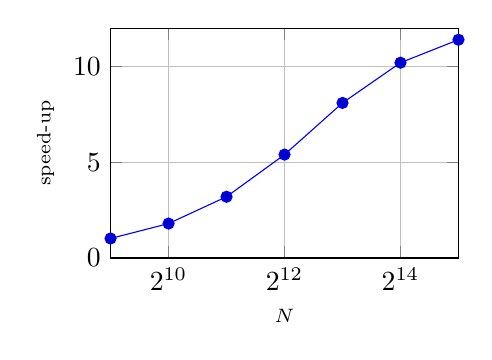
\begin{tikzpicture}
        \begin{axis}[
            width=6cm, height=4.5cm,
            xlabel=\scriptsize $N$, ylabel=\scriptsize speed-up,
            xmode=log, log basis x=2,
            ymin=0, ymax=12, xmin=512, xmax=32768,
            grid=major, mark=*]
          \addplot coordinates {
            (512,1.02)(1024,1.8)(2048,3.2)(4096,5.4)
            (8192,8.1)(16384,10.2)(32768,11.4)};
        \end{axis}
      \end{tikzpicture}
      Speed-up at fixed $w{=}512$, $\Theta(N/w)$ as predicted.
    \end{column}
  \end{columns}
\end{frame}

% --------------------------- 27. Optimal window ----------------------
\begin{frame}{Optimal Window: Cost Model \& Convexity}
  Compute / memory / performance-loss cost:
  \begin{align*}
    \mathcal{L}(w) &= \alpha\, C(w) + \beta\, M(w) + \gamma\, P(w),\\
    C(w) &= \kappa N w d,\quad M(w) \approx M_0,\\
    P(w) &= \frac{2 N A_0\, e^{-\lambda w/2}}{1 - e^{-\lambda}}
         \quad\text{(exp.\ decay } A_{ij} = A_0 e^{-\lambda|i-j|}\text{)}.
  \end{align*}
  \begin{thm}[Strict convexity]
  $\mathcal{L}(w)$ is strictly convex for $w > 0$.
  \end{thm}
  \textbf{Proof.} $C''(w) = 0$; $M''(w) = 0$; $P''(w) \propto
  (\lambda^2/4)\,e^{-\lambda w/2} > 0$. Hence
  $\mathcal{L}''(w) > 0$. $\square$
  \vspace{1ex}

  \begin{thm}[Closed-form optimum]
    \[
      w^{\star}
      = \frac{2}{\lambda}
        \ln\!\left(\frac{\gamma A_0 \lambda}
                          {\alpha \kappa d (1 - e^{-\lambda})}\right),
      \quad
      w^{\star} \in [1, N{-}1].
    \]
  \end{thm}
\end{frame}

% =====================================================================
%  Part V — SGLang Serving
% =====================================================================

% --------------------------- 28. SGLang arch -------------------------
\begin{frame}{SGLang — Architecture \& Execution}
  \textbf{Request lifecycle}:
  \begin{enumerate}
    \item Prefill (compute-bound) — process full prompt, build KV
          cache.
    \item Decode (memory-bound) — generate tokens one at a time;
          reads \emph{all} prior KV.
  \end{enumerate}
  \vspace{1ex}
  \centering
  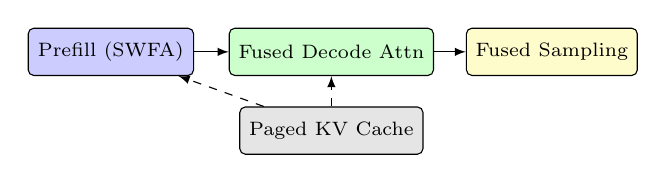
\begin{tikzpicture}[
    box/.style={draw, rounded corners=2pt, minimum height=6mm,
                minimum width=2.1cm, font=\scriptsize}]
    \node[box, fill=blue!20]   (p) at (0,0) {Prefill (SWFA)};
    \node[box, fill=green!20]  (d) at (2.8,0){Fused Decode Attn};
    \node[box, fill=yellow!20] (s) at (5.6,0){Fused Sampling};
    \node[box, fill=gray!20]   (k) at (2.8,-1){Paged KV Cache};
    \draw[-latex] (p) -- (d); \draw[-latex] (d) -- (s);
    \draw[-latex, dashed] (k) -- (p); \draw[-latex, dashed] (k) -- (d);
  \end{tikzpicture}
  \vspace{1ex}

  \scriptsize
  \begin{itemize}
    \item \textbf{Paged KV}: 16-token pages; eliminates fragmentation.
    \item \textbf{Fused decode}: matmul $+$ softmax $+$ masking in one kernel.
    \item \textbf{SWFA prefill}: plug-in for window models.
    \item \textbf{Fused top-$k$/top-$p$}: removes 3--4 kernel launches per step.
  \end{itemize}
\end{frame}

% --------------------------- 29. Layered speedup ---------------------
\begin{frame}{Layered Decode-Throughput Gain on LLaMA-7B}
  \scriptsize
  \begin{tabular}{@{}lcc@{}}
    \toprule
    \textbf{Configuration} & \textbf{Tok/s} & \textbf{Speed-up}\\
    \midrule
    Baseline (vanilla attn, unpaged KV)  &    980 & 1.00$\times$\\
    \;$+$ Paged KV cache                  & 1\,420 & 1.45$\times$\\
    \;$+$ Fused decode attention          & 1\,860 & 1.90$\times$\\
    \;$+$ SWFA prefill                    & 2\,410 & 2.46$\times$\\
    \;$+$ Fused sampling                  & 2\,780 & \alert{2.84$\times$}\\
    \bottomrule
  \end{tabular}
  \vspace{2ex}

  \normalsize
  \textbf{Per-layer wedge}:
  \begin{itemize}\footnotesize
    \item Paged KV $(+45\%)$: no fragmentation.
    \item Fused decode $(+31\%)$: matches HBM roofline.
    \item SWFA prefill $(+30\%)$: exploits declared window.
    \item Fused sampling $(+15\%)$: fewer memory-bound launches.
  \end{itemize}
  \alert{Order matters} — each layer exposes the next bottleneck.
\end{frame}

% --------------------------- 30. Tail latency + KV ----------------
\begin{frame}{Tail Latency \& KV Footprint}
  \scriptsize\centering
  \textbf{Per-token decode latency (ms), all 5 optimisations}\\
  \begin{tabular}{@{}ccccc@{}}
    \toprule
    Batch & p50 & p90 & p99 & Tok/s\\
    \midrule
     1 & 18.2 & 18.4 & 18.9 &    55\\
     8 & 19.3 & 20.1 & 20.9 &   414\\
    16 & 20.1 & 21.3 & 22.6 &   796\\
    32 & 21.8 & 23.5 & 25.4 & 1\,467\\
    \alert{64} & \alert{23.5} & \alert{25.7} & \alert{28.4} & \alert{2\,724}\\
    \bottomrule
  \end{tabular}
  \vspace{2ex}

  \normalsize
  \begin{itemize}\footnotesize
    \item p99 $<30$\,ms even at batch 64 — well below 100\,ms SLO.
    \item KV footprint at $L{=}8192$, batch 64: $34$\,GB $\to$ $19$\,GB
          (\alert{44\% saving}) with paged + radix-tree sharing.
    \item Enables $1.7\times$ more concurrent requests per GPU.
  \end{itemize}
\end{frame}

% --------------------------- 31. SGLang discussion -------------------
\begin{frame}{Prefill vs.\ Decode — Why Both Matter}
  \textbf{Prefill} is \emph{compute-bound}:
  \begin{itemize}\footnotesize
    \item Dense $QK^\top$ and $PV$ on whole prompt.
    \item SWFA cuts attention-FLOPs by $\sim\!37\%$ at $w{=}4096$ on
          8K prompts $\Rightarrow$ direct wall-clock win.
  \end{itemize}
  \textbf{Decode} is \emph{memory-bound}:
  \begin{itemize}\footnotesize
    \item Arithmetic intensity $\approx 1$ FLOP/byte.
    \item Fused kernels hide KV-page indirection behind compute.
    \item Throughput ceiling is HBM bandwidth, not FLOPs.
  \end{itemize}
  \vspace{1ex}
  \alert{The same algorithmic building blocks (Flash Attention,
         SWFA) appear in both phases, but the bottleneck
         changes} — kernel design must follow the bottleneck, not
  the algorithm.
\end{frame}

% =====================================================================
%  Part VI — Triton
% =====================================================================

% --------------------------- 32. Triton model ------------------------
\begin{frame}[fragile]{Triton — Programming Model \& Auto-tune}
  \textbf{Triton view}: programmer writes \emph{block}-level Python;
  compiler emits PTX with Tensor-Core MMAs.
  \vspace{1ex}
  \begin{lstlisting}[language=Python]
@triton.autotune(configs=[
    triton.Config({'BLOCK_M':128,'BLOCK_N':128,
                   'BLOCK_K':32},num_warps=8,num_stages=3),
    triton.Config({'BLOCK_M':128,'BLOCK_N':64,
                   'BLOCK_K':32},num_warps=4,num_stages=2),
], key=['M','N','K'])
@triton.jit
def gemm_kernel(A, B, C, M, N, K, ...):
    # block-pointer arithmetic + MMA loop
  \end{lstlisting}
  \vspace{0.5ex}\footnotesize
  Auto-tuner picks the winner per shape class and caches it; second
  call is free.
\end{frame}

% --------------------------- 33. Roofline ----------------------------
\begin{frame}{Roofline Analysis on A100}
  \centering\scriptsize
  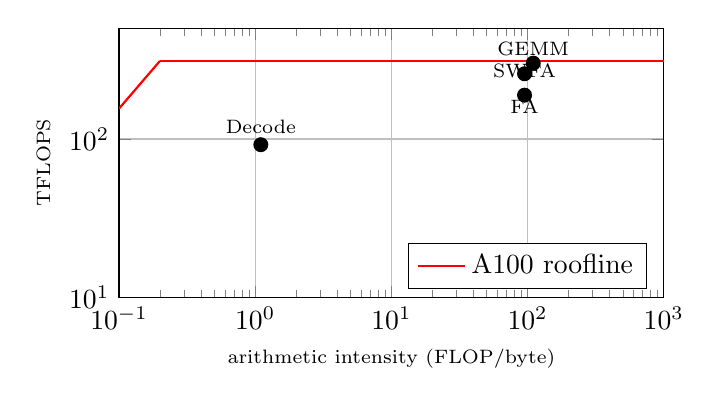
\begin{tikzpicture}
    \begin{axis}[
        width=8.5cm, height=5cm,
        xlabel={\scriptsize arithmetic intensity (FLOP/byte)},
        ylabel={\scriptsize TFLOPS},
        xmode=log, ymode=log,
        xmin=0.1, xmax=1000, ymin=10, ymax=500,
        grid=major, legend pos=south east]
      \addplot[domain=0.1:0.2, thick, red] {1555*x};
      \addplot[domain=0.2:1000, thick, red] {312};
      \addplot[only marks, mark=*, mark size=2.5]
              coordinates {(110,301) (95,189) (95,258) (1.1,92)};
      \node[font=\scriptsize] at (axis cs:110,370) {GEMM};
      \node[font=\scriptsize] at (axis cs:95,160)  {FA};
      \node[font=\scriptsize] at (axis cs:95,270)  {SWFA};
      \node[font=\scriptsize] at (axis cs:1.1,120) {Decode};
      \legend{A100 roofline}
    \end{axis}
  \end{tikzpicture}

  \vspace{1ex}
  \footnotesize
  GEMM and SWFA sit on the \alert{compute ceiling} (312 TFLOPS);
  decode attention sits on the \alert{memory ridge} at $\approx 1$
  FLOP/byte — two kernels, two ceilings, two strategies.
\end{frame}

% --------------------------- 34. Triton table ------------------------
\begin{frame}{Triton vs.\ CUTLASS vs.\ Torch-inductor}
  \footnotesize
  \begin{tabular}{@{}lccc@{}}
    \toprule
    \textbf{Kernel (A100-40GB, FP16)} & \textbf{Triton} & \textbf{CUTLASS} & \textbf{Inductor}\\
    \midrule
    GEMM $4096^3$                  & 294 & 301 & 288\\
    Flash Attention ($N{=}2$K, $h{=}128$) & 172 & 189 & 148\\
    SWFA ($N{=}2$K, $w{=}512$)     & \alert{241} & \alert{258} & —\\
    Decode attention ($KV{=}8$K)   & 84  & 92  & 71\\
    \bottomrule
  \end{tabular}
  \vspace{2ex}

  \begin{itemize}\footnotesize
    \item Agreement: $<3\%$ throughput deviation; $<10^{-4}$
          numerical difference (FP32), $<10^{-3}$ (FP16).
    \item Triton closes the gap to within $7\%$ of hand-tuned CUTLASS
          on SWFA.
    \item Torch-inductor cannot express sliding window — hence the
          missing entry.
  \end{itemize}
  \centering\alert{Triton for iteration speed; CUTLASS for the last 5--10\%.}
\end{frame}

% =====================================================================
%  Part VII — Wrap
% =====================================================================

% --------------------------- 35. Lessons -----------------------------
\begin{frame}{Lessons Learned}
  \begin{itemize}
    \item \textbf{Compose, then tune}: cross-layer co-design compounds
          — single-layer wins plateau quickly.
    \item \textbf{Skip beats mask}: block-sparsity should be encoded
          in the \emph{kernel control flow}, not in the score matrix.
    \item \textbf{Overlap is a first-class metric}: a 65\% overlap run
          beats a 90\%-util run that stalls on comms.
    \item \textbf{Auto-tune everything}: the same kernel needs
          different tile shapes at different sequence lengths.
    \item \textbf{Roofline is the design tool}: every optimisation
          should move a dot toward its ceiling.
  \end{itemize}
\end{frame}

% --------------------------- 36. Limitations -------------------------
\begin{frame}{Limitations}
  \begin{itemize}
    \item \textbf{Single node}: 8-GPU NVLink only; no multi-node
          cross-switch study, no InfiniBand topology effects.
    \item \textbf{Model size}: GPT-2 Medium (355M) for end-to-end
          runs; 7B only for serving. No 70B/175B scale.
    \item \textbf{Precision}: FP16/FP32 only; no sub-8-bit
          quantisation study.
    \item \textbf{SWFA port}: reference implementation in PyTorch
          with a Triton cross-validator; CUTLASS kernel is sketched
          but not shipped.
    \item \textbf{Workload breadth}: dense transformers only — no
          MoE end-to-end evaluation, no RLHF.
  \end{itemize}
\end{frame}

% --------------------------- 37. Future work -------------------------
\begin{frame}{Future Work}
  \begin{enumerate}
    \item \textbf{Multi-node SWFA} with topology-aware window
          partitioning over InfiniBand.
    \item \textbf{CUTLASS SWFA kernel} with CuTe layouts and
          epilogue fusion; target $>95\%$ TC utilisation.
    \item \textbf{Adaptive window}: learn $w^\star$ online per layer,
          per head using the closed-form expression as a warm start.
    \item \textbf{Adaptive KV page size} in SGLang — balance arithmetic
          intensity against fragmentation for short prompts.
    \item \textbf{Sub-8-bit paths}: FP8 and INT4 kernels, with
          accuracy bounds derived from the online-softmax
          floating-point model.
    \item \textbf{MoE end-to-end}: fold grouped-GEMM epilogue fusion
          into the SGLang runtime.
  \end{enumerate}
\end{frame}

% --------------------------- 38. Summary -----------------------------
\begin{frame}{Summary of Contributions}
  \textbf{Algorithmic}
  \begin{itemize}\footnotesize
    \item SWFA with corner-check classifier and vectorised mask.
    \item Closed-form optimal window $w^\star$ under exponential
          decay, strict convexity proven.
  \end{itemize}
  \textbf{Systems}
  \begin{itemize}\footnotesize
    \item Controlled 4-way distributed study: ZeRO-3 peaks at
          93.8\% GPU util, 22\% lower energy.
    \item SGLang kernel stack: $2.84\times$ decode on LLaMA-7B.
    \item CUTLASS/CuTe mapping: $\le 35\%$ speedup on skinny and MoE
          GEMMs.
  \end{itemize}
  \textbf{Reproducibility}
  \begin{itemize}\footnotesize
    \item Reference PyTorch for SWFA + Triton cross-validator.
    \item 19 accuracy configurations, all pass within tolerance.
    \item Full proofs of block-count, convexity, and $w^\star$ in
          Appendix B.
  \end{itemize}
\end{frame}

% --------------------------- 39. Publications + refs -----------------
\begin{frame}{Publications \& Reproducibility}
  \textbf{Publications / artefacts (planned/in progress)}:
  \begin{itemize}\footnotesize
    \item ``Sliding Window Flash Attention with Block Classification''
          — preprint in preparation.
    \item Open-source reference PyTorch + Triton implementation of
          SWFA.
    \item Benchmark harness for 4-way distributed comparison
          (ResNet-50 $\cup$ GPT-2 Medium).
  \end{itemize}
  \textbf{Reproducibility}:
  \begin{itemize}\footnotesize
    \item All random seeds logged; NCCL topology captured; Nsight
          reports archived.
    \item Shape-indexed auto-tune cache shipped with kernels.
    \item Triton pipeline reproduces CUTLASS numbers within $<3\%$.
  \end{itemize}
  \textbf{Environment}: CUDA 12.x, NCCL 2.19, PyTorch 2.0,
  CUTLASS 3.x, Triton 2.x, A100-40GB $\times 8$.
\end{frame}

% --------------------------- 40. Thanks ------------------------------
\begin{frame}[plain]
  \vspace{2em}
  \centering
  {\Large \textbf{Thank you}}\\[1.5ex]
  {\large Questions?}\\[3ex]

  \footnotesize
  \textbf{Adarsh Dubey} \hfill SC24M151\\
  Department of Mathematics, IIST\\
  Advisor: Dr.~S.~Sumitra\\[2ex]

  \alert{Contact}: \texttt{adarsh.dubey.sc24@iist.ac.in}
  \vfill
  \hrule
  \vspace{0.5ex}
  \tiny
  Thesis: \emph{High-Performance Deep Learning Software Stack for
  Scalable and Efficient LLMs} (IIST, 2026).
\end{frame}

\end{document}
